% original file written by Stephanie Jachner
%% English version based on original SALMO documentation of Juergen Benndorf
%% with some adaptions of Thomas Petzoldt

\documentclass[11pt,a4paper]{article}
\usepackage[T1]{fontenc}
\usepackage[ansinew]{inputenc}
\usepackage[fleqn]{amsmath}
\usepackage{amsfonts}
\usepackage{mathptmx}
\usepackage{longtable}
\usepackage{natbib}
\usepackage{hyperref}

\setlength{\parindent}{0em}          \parskip7pt plus1pt minus2pt
\setlength{\mathindent}{0cm}

 \author{The SALMO Developer Group\\ Technische Universit\"at Dresden\\
 Institute of Hydrobiologie\\ \url{http://www.tu-dresden.de/hydrobiologie}}
\title{Parameters and Equations of the Lake Model SALMO}
%\VignetteIndexEntry{Parameters and Equations of the Lake Model SALMO}

\usepackage{Sweave}
\begin{document}

\maketitle

\tableofcontents

\section{The lake model SALMO}

The ``Ecological Lake Model SALMO'' (Simulation by means of an
Analytical MOdel) is a dynamic model, originally developed at TU Dresden,
Institute of Hydrobiology. It describes essential parts of the aquatic foodweb
of lakes and reservoirs.

The system of ordinary differential equations originates from the
habilitation thesis of \citet{Benndorf1979a} who modelled annual
time-dependend development of phytoplankton (two groups), zooplankton,
oxygen, nutrients (N and P) and external detritus of the water body,
based on field observations and laboratory experiments.  First
implementations in Fortran and HPL (Hewlett Packard Language) have
been developed by Recknagel \citep{Recknagel1980, Recknagel1982} and
used for several theoretical and practical studies
\cite[e.g.,][]{Benndorf1979b,Benndorf1979c,Benndorf1982,Benndorf1985a,Petzoldt1991}.

Since then, several versions, implementations and spin-offs followed.

This R package aims to make an ``almost original version'' of the
model publicly available under the GPL 2 and to foster further
development.  Its source code is based on an independent
implementation from the system of equations of model version SALMO II
\citep{Benndorf1988}.  The JAVA version of Dietze and Planke
\citep{Willmitzer1998} was the followed by the C version SALMO-1D of
Rolinski \citep{Petzoldt2002,Rolinski2005,Petzoldt2005,Petzoldt2006},
that allowed coupling to hydrophysical models such as LAKE
\citep{Baumert1989,Baumert2005a,Baumert2005awrl} or GOTM
\citep{Umlauf2007}. During this time, the system equations underwent
slow but steady evolution and generalisation.

Recently, \citet{Sachse2014} coupled SALMO-1D to a macrophyte module
based on the model PCLake \citep{Janse1995,Janse1998} to simulate
growth of and interaction effects with submersed water plants.

\begin{figure}
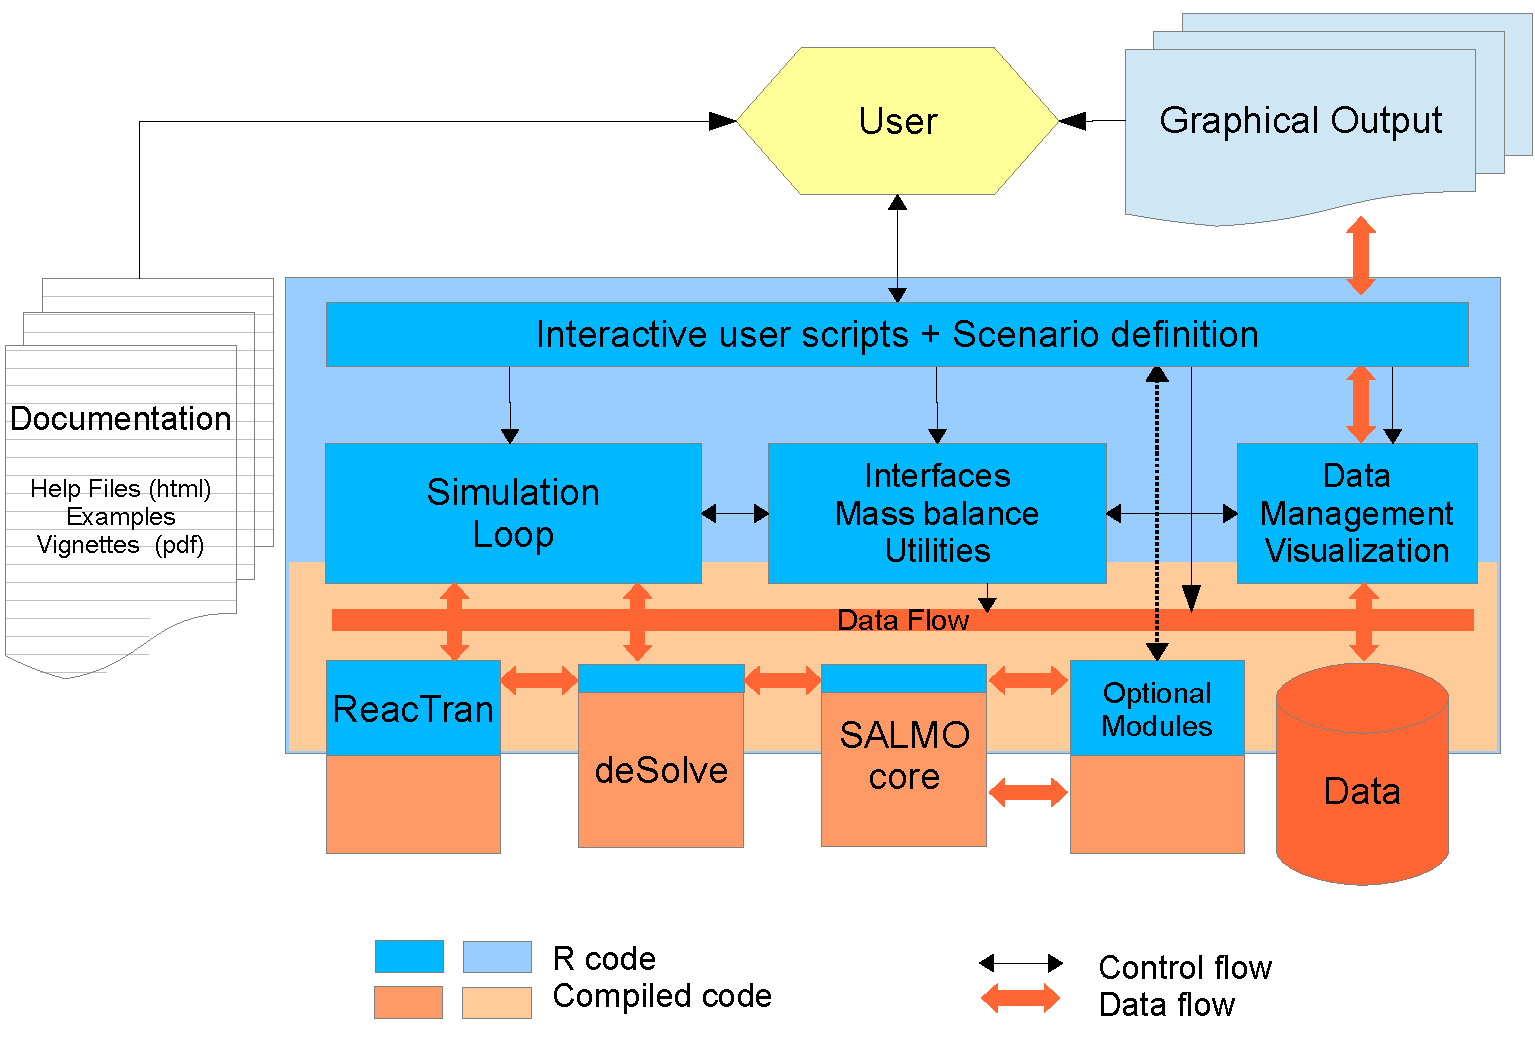
\includegraphics[width=\textwidth]{rsalmo.pdf}
\caption{\label{fgrsalmo} Concept of the R package rSALMO}
\end{figure}

\begin{figure}
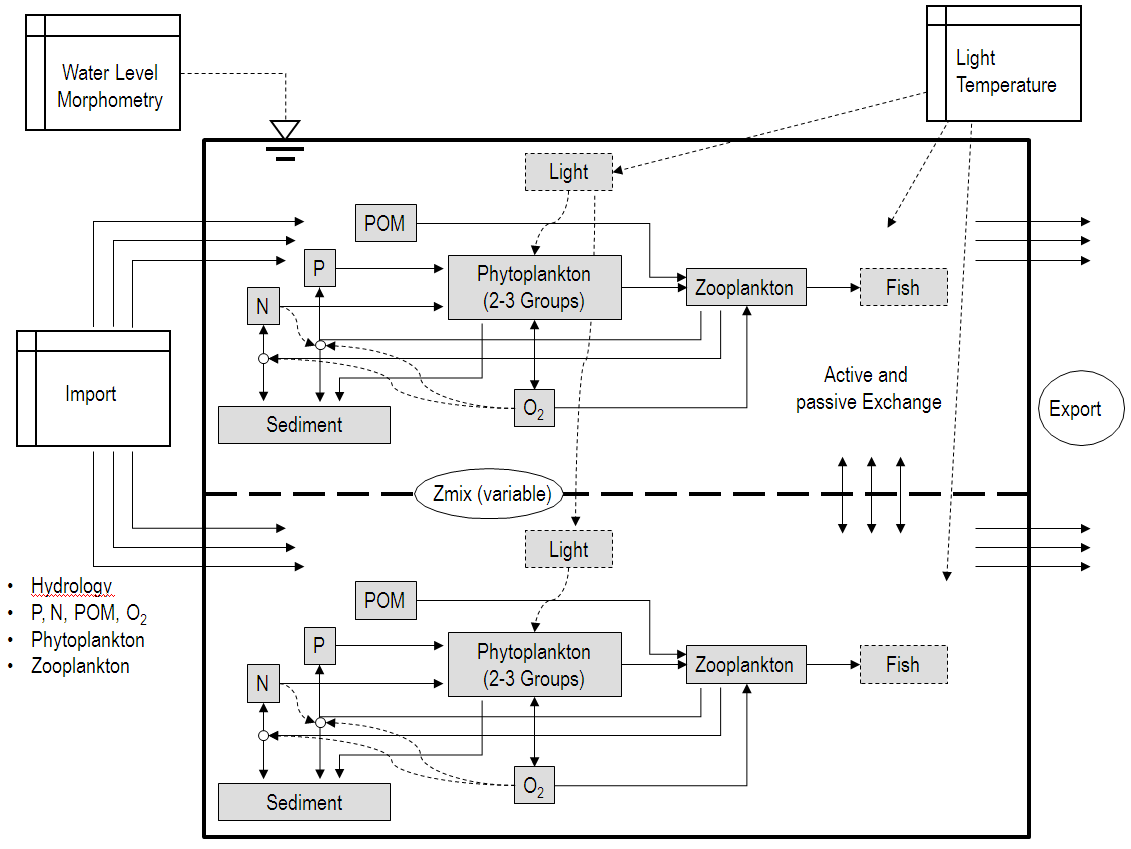
\includegraphics[width=\textwidth]{salmo-2.png}
\caption{\label{fgsalmo} Simplified schematic representation of the two-layer
configuration of lake model SALMO-2}
\end{figure}



The code is now maintained by Thomas Petzoldt at TU Dresden, Institute
of Hydrobiology. More information can be found on:

\begin{itemize}
  \item \url{http://www.simecol.de/salmo/}
  \item \url{http://rlimnolab.r-forge.r-project.org/}
  \item \url{http://tu-dresden.de/Members/thomas.petzoldt/}
\end{itemize}

Note that this is still work in progress, so please contact me before
trying to run applications or investing your valuable work.

\section{Model parameters and internal variables}


\subsection{Constant model parameters}

\begin{longtable} {l p{9.5cm}}
 $ANSFMIN = 0.01$ & minimal value of $ansf$ (release of inorganic nitrogen
 from sediment) at 0 �C ($g$ $N$ $m^{-2}$ $d^{-1}$)\\
 $APSFMAX = 7$ & maximal value of $apsf$ (phosphorus release from sediment),
   if oxygen concentration $o < LINDEN$ ($mg$ $P$ $m^{-2}$ $d^{-1}$)\\
 $APSFMIN = 1$ & minimal value of $apsf$  (phosphorus release from sediment),
   at saturation concentration of oxygen ($mg$ $P$ $m^{-2}$ $d^{-1}$)\\
 $AZMAX = 0.8$ & maximal assimilation coefficient of zooplankton at very low ingestion rate (-)\\
 $AZMIN = 0.4$ & minimal assimilation coefficient at ($g=GMAX$) (-)\\
 $DTA = 3.9$ & parameters of the empirical relationship between egg development time
   of crustaceans and temperature (-)\\
 $DTB = 0.15$ & cf. DTA\\
 $DTC = 0.26$ & cf. DTA\\
 $DTMIN = 5$ & minimum value of egg development time of the crustaceans
   below of which the egg development time is neglected in the calculation of zooplankton growth ($d$)\\
 $EPSD = 0.023$ & specific light extinction coefficient of detritus ($m^2$ $g^{-1}$)\\
 $GI = 0.8$ & inhibition factor of the ingestion rate due to light (-)\\
 $GMAX = 1.3$ & maximum value of $g$ (specific ingestion rate of zooplankton) ($g$ $g^{-1}$ $d^{-1}$)\\
 $GMIN = 0.26$ & minimum value of $g$ (specific ingestion rate of zooplankton) near 0 �C ($g$ $g^{-1}$ $d^{-1}$)\\
 $KANSF = 0.004$ & slope of the function $ansf(temp)$ (release of organic nitrogen from sediment) ($g$ $m^{-2}$ $d^{-1}$ �$C^{-1}$)\\
 $KAPSF = 1.25$ & half saturation constant of the inverse function $apsf(o)$
 (phosphorus release from sediment) ($g$ $O_2$ $m^{-3}$)\\
 $KDEN = 0.045$ & parameter of the dependence of denitrification on the supply of organic matter ($g$ $cm^{-3}$)\\
 $KMINER = 0.04$ & mineralisation constant related to oxygen consumption by sinking phytoplankton ($d^{-1}$)\\ % hypolimnion ??
 $KMO = 0.35$ & half saturation constant of the dependence of zooplankton mortality on zooplankton biomass ($g$ $m^{-3}$)\\
 $KPSED = 0$ & specific scenario parameter for hard water lakes, sedimentation of phosphate by co-precipitation
   with calcite as daily percentage of the in-lake phosphate (-)\\ % check 'percentage' !!
 $KSEZA = 2.5$ & oxygen concentration $o$, which causes 50\% of the maximal oxygen consumption by the sediment ($g$ $O_2$ $m^{-3}$)\\
 $KSRFMAX = 4.3$ & critical value of $ksrf$ (corrected strong rain factor), above
  the underwater light climate is reduced due to erosion-induced turbidity (-)\\
 $KXG = 5$ & half saturation constant of the relationship between ingestion rate of zooplankton and food ($g$ $m^{-3}$)\\
 $KXMIN = 2.5$ & theoretical minimum of $kx$ and $kxn$ (half saturation constant of the inverse
   relationship between photosynthesis rate and biomass of phytoplankton at nitrogen limitation of phytoplankton growth) ($g$ $m^{-3}$)\\
 $KZMIN = 4$ & theoretical minimum value of $kz$ (half saturation value of the inverse relationship
   between ingestion rate and biomass of zooplankton) ($g$ $m^{-3}$)\\
 $LGH = 0.4$ & parameter of the dependence of the half saturation value $kz_i$ on
   phytoplankton biomass at high biomass of $x_i$ (-)\\
 $LGL = 5.76$ & parameter of the dependence of the half saturation value $kz_i$ on
    phytoplankton biomass at low biomass of $x_i$ (-)\\
 $LINDEN = 1$ & oxygen threshold below which denitrification occurs ($g$ $O_2$ $m^{-3}$)\\
 $LXH = 0.1$ & parameter of the dependence of the half saturation value $kx$
 on the phosphate concentration at high phosphate concentration (-)\\
 $LXHN = 209.56$ & parameter of the dependence of the half saturation value 
 $kxn$  on the concentration of inorganic nitrogen at high inorganic nitrogen concentration  (-)\\
 $LXL = 2.78$ &  parameter of the dependence of the half saturation value $kx$ on
  on the phosphate concentration at low phosphate concentration(-)\\
 $LXLN = 19.04$ & parameter of the dependence of the half saturation value 
 $kxn$ on the concentration of inorganic nitrogen at low inorganic nitrogen concentration (-)\\
 $MGH = 1.5$ & parameter of the dependence of the half saturation value  $kz$ on phytoplankton biomass at high biomass of phytoplankton (-)\\
 $MGL = 0.41$ & parameter of the dependence of the half saturation value  $kz$  on phytoplankton biomass at low biomass of phytoplankton (-)\\
 $MOMIN = 0.015$ & rate of zooplankton mortality near 0 �C at zooplankton biomass
 $z$ much higher than $KMO$ ($d^{-1}$)\\
 $MOT = 0.006$ & slope of the function $mortz(temp)$ (�$C$ $d^{-1}$)\\
 $MXH = 1.55$ & parameter of the dependence of the half saturation value  $kx$ on the phosphate concentration at high phosphate concentration  (-)\\
 $MXL = 0.39$ & parameter of the dependence of the half saturation value  $kx$ on the phosphate concentration at low phosphate concentration  (-)\\
 $OPTNP = 0.0072$ & optimum $N$/$P$ mass ratio (-)\\
 $PF = 1$ & preference factor for ingestion of detritus by zooplankton (-)\\
 $R = 2$ & parameter of the dependence of the ingestion rate of zooplankton on water temperature (-)\\
 $RAT = 0.7$ & ratio of soluble to total phosphorus in zooplankton faeces (-)\\
 $RATF = 0.7$ & ratio of soluble to total phosphorus in fish excrements and during remineralization of dead zooplankton (-)\\
 $RATN = 0.7$ &  ratio of soluble to total nitrogen in zooplankton faeces (-)\\
 $RATNF = 0.7$ & ratio of soluble to total nitrogen in fish excrements and during remineralization of dead zooplankton  (-)\\
 $RL = 0.9$ & factor for light reflection at the water surface (-)\\
 $RLW = 0.2$ &  factor for light reflection at the water during winter stagnation (ice cover) (-)\\
 $RXMF = 0.3$ & fraction of the gross photosynthesis rate which is consumed by respiration additionally to the basis respiration (-)\\
 $RZMIN = 0.08$ & respiration rate of zooplankton at optimal temperature for feeding but without food supply ($d^{-1}$)\\
 $RZOPT = 0.22$ & respiration rate of zooplankton at optimal temperature for feeding and maximum ingestion rate ($d^{-1}$)\\
 $RZTMIN = 0.05$ & respiration rate of zooplankton near O �C and optimal food supply ($d^{-1}$)\\
 $SF = 1.0$ & heuristic sediment fucussing parameter (-)\\
 $SEZMAX = 0.4$ & maximum oxygen consumption by the sediment ($g$ $O_2$ $m^{-3} d^{-1}$)\\
 $EPSR = 0.2668$ & specific light extinction coefficient due to turbidity and erosion at strong rain events ($m^2$ $g^{-1}$)\\
 $TOPTZ = 20$ & optimal temperature for feeding activity of the zooplankton (�$C$)\\
 $UXZD = 0.75$ & factor of the physiological utilisation of detritus by zooplankton (-)\\
 $VD = 0.2$ & net sinking velocity of detritus ($m$ $d^{-1}$)\\
 $VMIG = 0.15$ & net migration velocity of zooplankton from hypolimnion to epilimnion ($m$ $d^{-1}$)\\ % check if necessary in 1D model !!
 $WPKX = 12.5$ & point of inflexion of the function $kx(p)$ ($mg$ $m^{-3}$)\\
 $WPKZ = 8.6$ &  point of inflexion of the function $kz(x)$ ($g$ $m^{-3}$)\\
 $YD = 2$ & phosphorus related `yield' coefficient of detritus ($g$ wet weight/$mg$ $P$)\\ % thpe: g changed to mg !!
 $YND = 285$ & nitrogen related `yield' coefficient of detritus ($g$ wet weight/$g$ $N$)\\
 $YNX = 57$ & nitrogen related yield coefficient of phytoplankton ($g$ wet weight /$g$ $N$)\\
 $YOX = 3.75$ & oxygen equivalent of the biomass ($g$ wet weight/$g$ $O_2$)\\
 $YZN = 110$ & nitrogen related yield coefficient of zooplankton ($g$ wet weight/$g$ $N$)\\
 $YZP = 0.8$ & phosphorus related yield coefficient of phytoplankton ($g$ wet weight/$mg$ $P$)\\
\end{longtable}

\subsection{Phytoplankton parameters}

\begin{longtable} {l p{9.5cm}}
 $EPSX= (0.0368, 0.046, 0.046)$ & specific light extinction coefficient of phytoplankton group
 $i$ ($m^2$ $g^{-1}$)\\
 $KI = (28, 29, 29)$ & half saturation constant of the dependence of the photosynthesis rate of phytoplankton group $i$ on light ($J$ $cm^{-2}$ $d^{-1}$)\\
 $KN = (0.0123, 0.0123, 0.0095)$ & half saturation constant of the dependence of the photosynthesis rate of phytoplankton group $i$ on nitrogen at minimal phytoplankton biomass ($g$ $N$ $m^{-3}$)\\
 $KP = (1.7, 1.7, 9.5)$ & half saturation constant of the dependence of the photosynthesis rate of phytoplankton group $i$ on phosphorus at minimal phytoplankton biomass 
 ($g$ $N$ $m^{-3}$)\\
 $KPF = (1.1, 4, 0)$ & half saturation value of the dependence of the preference factor of zooplankton $pf_i$ for phytoplankton group $i$ on availability of the other groups ($g$ $m^{-3}$)\\ % % check this !! Rene??
 $PFC = (0, 0.3, 1)$ & preference factor for ingestion of phytoplankton by zooplankton (-)\\
 $PFX = (0.1, 3, 0)$ & threshold of the other phytoplankton groups above which $pf_i$ is decreasing ($g$ $m^{-3}$)\\
 $PHOTXMAX = (1.7, 1.8, 3.5)$ & maximum value of $photx_i$ (gross photosynthesis rate of group $i$) at optimal conditions ($d^{-1}$)\\
 $PHOTXMIN = (0, 0.17, 0.35)$ & values of $photx_i$ near to 0 �C at optimal light and nutrient conditions ($d^{-1}$)\\
 $RXTMIN = (0, 0.02, 0.02)$ & rate of basis respiration of phytoplankton group $i$ near 0 �C ($d^{-1}$)\\
 $RXTOPT = (0.057, 0.06, 0.06)$ & rate of basis respiration of phytoplankton group $i$
  at the group specific optimum temperature ($d^{-1}$)\\
 $TOPTX = (25, 20, 25)$ & optimum temperature for phytoplankton group $i$ (�$C$)\\
 $UXZ = (1, 1, 1)$ & factor of the physiological utilisation of phytoplankton group 
 $i$ by zooplankton (-)\\
 $VS = (0.05, 0.1, 0.1)$ & net sinking velocity of phytoplankton group $i$ ($m$ $d^{-1}$)\\
 $YX = (1, 0.8, 0.41)$ & phosphorus related yield coefficient of phytoplankton group $i$ ($g$ wet weight / $mg$ $P$)\\
\end{longtable}

\clearpage

\subsection{Internal variables of the model}


\begin{longtable} {l p{13cm}}
 $ansf$ & release rate of anorganic nitrogen from sediment ($g$ $N$ $m^{-2}$ $d^{-1}$)\\
 $apsf$ & release rate of anorganic phosphorus from sediment  ($mg$ $P$ $m^{-2}$ $d^{-1}$)\\
 $assiz$ & assimilation rate of zooplankton ($g$ $g^{-1}$ $d^{-1}$)\\
 $az$ & assimilation coefficient ($g$ food assimilated / $g$ food ingested)\\
 $bd$ & sedimentation rate of detritus ($d^{-1}$)\\
 $bx_i$ & sedimentation rate of phytoplankton group $i$ ($d^{-1}$)\\
 $dgraz$ & loss of detritus by zooplankton grazing ($g$ $m^{-3}$ $d^{-1}$)\\
 $dt$ & egg development time of all crustaceans ($d$)\\
 $egg$ & reduction factor of the zooplankton growth rate due to low reproduction (-)\\
 $eps$ & extinction coefficient of light (photosynthetic active radiation between 400 and 700 nm) ($m^{-1}$)\\
 $g$ & specific ingestion rate of zooplankton ($g$ $g^{-1}$ $d^{-1}$)\\
 $g_i$ & specific ingestion rate of phytoplankton group $i$ by zooplankton ($g$ $g^{-1}$ $d^{-1}$)\\ % ?? GI = light inhibition ??
 $g3d$ & specific ingestion rate of detritus by zooplankton ($g$ $g^{-1}$ $d^{-1}$)\\ % !! check this
 $gdb$ & term of the dependence of the ingestion rate in the dark on the biomass of the phyto- and zooplankton (-)\\
 $gdt$ & temperature term of the ingestion rate in the dark ($g$ $g^{-1}$ $d^{-1}$)\\
 $gl$ & specific ingestion rate of zooplankton $g$ in the light ($g$ $g^{-1}$ $d^{-1}$)\\
 $hl$ & light hours per day (photo period) ($h$ $d^{-1}$)\\
 $hwg_i$ & auxillary value for the calculation of the ingestion rate $g_i$ ($g$ $g^{-1}$ $d^{-1}$)\\
 $hwgd$ &  auxillary value for the calculation of $gd$ ($g$ $g^{-1}$ $d^{-1}$)\\
 $hwgd_i$ &  auxillary value for the calculation of  $gd$ ($g$ $g^{-1}$ $d^{-1}$)\\
 $hwgdb_i$ &  auxillary value for the calculation of  $gdb$ (-)\\
 $hwgdbd$ &  auxillary value for the calculation of  $gdb$ (-)\\
 $hwgdd$ &  auxillary value for the calculation of  $gd$ ($g$ $g^{-1}$ $d^{-1}$)\\
 $hwgl_i$ &  auxillary value for the calculation of  $gd$ and $gl$ ($g$ $g^{-1}$ $d^{-1}$)\\
 $hwgld$ &  auxillary value for the calculation of  $gd$ and $gl$ ($g$ $g^{-1}$ $d^{-1}$)\\
 $ired$ & value of $iin$ (incoming radiation) reduced by reflection ($J$ $cm^{-2}$ $d^{-1}$)\\
 $iredz$ & photosynthetic active light in depth $zvonj$ ($J$ $cm^{-2}$ $d^{-1}$)\\
 $ksrf$ & corrected factor for strong rain events or melting snow (correction with respect to reduced erosion
   in the drainage basin in dependence of the vegetation cover) (-)\\
 $kx$ & half saturation value of the inverse relationship between photosynthesis rate and phytoplankton biomass at phosphate limiting conditions ($g$ $m^{-3}$)\\
 $kxn$ &  half saturation value of the inverse relationship between photosynthesis rate and phytoplankton biomass at nitrogen limiting conditions  ($g$ $m^{-3}$)\\
 $kz$ & half saturation value of the inverse relationship between ingestion rate of zooplankton and zooplankton biomass ($g$ $m^{-3}$)\\
 $kz_i$ & half saturation value of the inverse relationship between ingestion rate of zooplankton and phytoplankton biomass of group $i$ ($g$ $m^{-3}$)\\
 $kzd$ & half saturation value of the inverse relationship between ingestion rate of zooplankton and detritus ($g$ $m^{-3}$)\\
 $lo$ & loading of the water body with oxygen-consuming organic matter
 ($g$ $m^{-3}$ $d^{-1}$)\\
 $lsez$ & loading of the water body due to to oxygen consumption by the sediment ($g$ $m^{-3}$ $d^{-1}$)\\
 $M$ & number of depth levels for the internal calculation of light and photosynthesis\\ % !! check this
 $miner_i$ & mineralisation coefficient related to oxygen consumption by sinking phytoplankton of group $i$ (-)\\
 $minerd$ &  mineralisation coefficient related to oxygen consumption by sinking detritus (-)\\
 $mortz$ & zooplankton mortality rate ($d^{-1}$)\\
 $nexkr$ & rate of nitrogen remineralisation by living zooplankton ($g$ $N$ $m^{-3}$ $d^{-1}$)\\
 $nkons$ & assimilation of inorganic nitrogen by phytoplankton ($g$ $N$ $m^{-3}$ $d^{-1}$)\\
 $nmort$ & rate of nitrogen mineralisation from dead zooplankton and by fish
 ($g$ $N$ $m^{-3}$ $d^{-1}$)\\
 $nrem$ & remineralisation of nitrogen ($g$ $N$ $m^{-3}$ $d^{-1}$)\\
 $nsf$ & release of inorganic nitrogen from the sediment to the water body
 ($g$ $N$ $m^{-3}$ $d^{-1}$)\\
 $o$ & state variable: oxygen concentration ($g$ $m^{-3}$)\\
 $okons$ & oxygen consumption (without phytoplankton respiration) ($g$ $m^{-3}$ $d^{-1}$)\\
 $oprod$ & net oxygen production by living phytoplankton ($g$ $m^{-3}$ $d^{-1}$)\\
 $pexkr$ & rate of phosphate remineralisation by zooplankton excretion ($mg$ $P$ $g$ $Z^{-1}$ $d^{-1}$)\\
 $pf_i$ & preference factor for ingestion of phytoplankton group $i$ by zooplankton (-)\\
 $photx_i$ & gross photosynthesis rate of phytoplankton group $i$ ($d^{-1}$)\\
 $phoxl_i$ & term of the relationship between photosynthesis rate of phytoplankton group $i$ and light (-)\\
 $phoxn_i$ & term of the relationship between photosynthesis rate of phytoplankton group  $i$ and
 anorganic nitrogen (including dependence on phytoplankton biomass) (-)\\
 $phoxns_i$ & term of the relationship between photosynthesis rate of phytoplankton group $i$ and
   the primary limiting nutrient(including dependence on phytoplankton biomass)
 (-)\\
 $phoxp_i$ & term of the relationship between photosynthesis rate of phytoplankton group $i$ and
   phosphate (including dependence on phytoplankton biomass) (-)\\
 $phoxt_i$ & term of the relationship between photosynthesis rate of phytoplankton group $i$ and
   temperature ($d^{-1}$)\\
 $pkons$ & phosphate consumption by phytoplankton ($mg$ $m^{-3}$ $d^{-1}$)\\
 $pmort$ & rate of phosphate remineralisation from dead zooplankton or zooplankton eaten by fish ($d^{-1}$)\\
 $prem$ & remineralisation of phosphate ($mg$ $m^{-3}$ $d^{-1}$)\\
 $psed$ & sedimentation of phosphate by coprecipitation with calcite or other minerals
 ($mg$ $m^{-3}$ $d^{-1}$)\\
 $psf$ & release of phosphorus from sediment to the water body ($mg$ $m^{-3}$ $d^{-1}$)\\
 $rx_i$ & respiration rate of phytoplankton group $i$ ($d^{-1}$)\\
 $rxt_i$ & base respiration rate of phytoplankton group $i$ ($d^{-1}$)\\
 $rz$ & respiration rate of zooplankton ($d^{-1}$)\\
 $rzg$ & factor of zooplankton respiration rate\\ % ?? for grazing ?
 $rzt$ & factor of zooplankton respiration rate\\ % ?? for temperature
 $sat$ & oxygen concentration at 100\% saturation ($g$ $m^{-3}$)\\
 $seza$ & oxygen consumption of the sediment (per sediment surface area) ($g$ $m^{-2}$ $d^{-1}$)\\
 $sumxpf$ & Summe der Zust�nde $x_i$ multipliziert mit $pf_i$\\
 $wx_i$ & growth rate of phytoplankton group $i$ ($d^{-1}$)\\
 $wz$ & growth rate of zooplankton ($d^{-1}$)\\
 $xgraz_i$ & phytoplankton loss of group $i$ due to zooplankton grazing ($g$ $m^{-3}$ $d^{-1}$)\\
 $xwa_i$ & growth of phytoplankton group $i$ ($g$ $m^{-3}$ $d^{-1}$)\\
 $zmo$ & zooplankton mortality ($g$ $m^{-3}$ $d^{-1}$)\\
 $zvonj$ & depth of layer $j$ ($m$)\\
 $zwa$ & zooplankton growth ($g$ $m^{-3}$ $d^{-1}$)\\
\end{longtable}

\clearpage

\section{SALMO - System of Equations}
\subsection{Anorganic Nitrogen}

Change =\\
- assimilation of organic nitrogen by phytoplankton\\
+ remineralisation of nitrogen\\
+  release of nitrogen from the sediment\\
+ \ldots

\begin{align*}
1.0 \hspace{0.5cm} \frac{dn}{dt}= -nkons+nrem+nsf+nden
\hspace{1.5cm} \left[\frac{gN}{m^3} \cdot d\right]
\end{align*}

\begin{align*}
1.2 \hspace{0.5cm} nkons=\sum \left(\frac{wx_i}{YNX} \cdot
x_i\right) + \frac{assiz}{YZN} \cdot RATN \cdot z \hspace{0.1cm};
\hspace{0.3cm} i=1,\ldots,nx
\end{align*}

\begin{align*}
1.3 \hspace{0.5cm} nrem=(nmort+nexkr) \cdot z
\end{align*}

\begin{align*}
1.4 \hspace{0.5cm} nmort = \frac{mortz \cdot RATNF}{YZN}
\end{align*}

\begin{align*}
1.5 \hspace{0.5cm} nexkr = \left(\left(\sum\frac{g_i}{YNX}\right)+
\frac{g_d}{YND} + \frac{rz}{YZN}\right) \cdot RATN \hspace{0.1cm};
\hspace{0.3cm} i=1,\ldots,xn
\end{align*}

\begin{align*}
1.7 \hspace{0.5cm} nsf = \frac{ansfq-ansfs}{v} \cdot ased
\end{align*}

\begin{align*}
1.8 \hspace{0.5cm} ansfs &=
 \begin{cases}
  NDSMAX \cdot \displaystyle \frac{n}{KNDS+n}
  \cdot KNDST^{\displaystyle (temp-4)} \hspace{0.1cm};
  & NDSSTART \leq t < NDSEND\\
  ANSFMIN + KANSF \cdot temp \hspace{0.1cm}; &
  \text{sonst}
 \end{cases}\\
ansfq &=
 \begin{cases}
  ANSFMIN \hspace{0.1cm}; & NDSSTART \leq t < NDSEND\\
  0 \hspace{0.1cm}; & \text{sonst}
 \end{cases}
\end{align*}

\begin{align*}
3.8 \hspace{0.5cm} nden = \frac{n \cdot KDEN \cdot lo}{KNDS + n}
\hspace{0.1cm}; \hspace{0.3cm} n > 0, \hspace{0.1cm} 0 \leq LINDEN
\end{align*}

\subsection{Dissolved Inorganic Phosphorus}

Change =\\
- phosphate uptake by phytoplankton\\
+ remineralisation\\
+ \ldots\\
+ release of phosphate from sediment

\begin{align*}
4.0 \hspace{0.5cm} \frac{dp}{dt} = -pkons + prem + presp + psf
\hspace{0.1cm} \hspace{1.5cm} \left[\frac{mg}{m^3} \cdot d\right]
\end{align*}

\begin{align*}
4.3 \hspace{0.5cm} pkons = \sum \left(\frac{photx_i}{YX_i} \cdot
x_i\right) + \frac{assiz}{YZP} \cdot RAT \cdot z \hspace{0.1cm};
\hspace{0.3cm} i=1,\ldots,nx
\end{align*}

\begin{align*}
4.4 \hspace{0.5cm} prem = (pmort + pexkr) \cdot z
\end{align*}

\begin{align*}
presp = \sum \left(\frac{rx_i}{YX_i} \cdot x_i \right)
\hspace{0.1cm}; \hspace{0.3cm} i=1,\ldots,nx
\end{align*}

\begin{align*}
4.5 \hspace{0.5cm} pmort = \frac{mortz \cdot RATF}{YZP}
\end{align*}

\begin{align*}
4.6 \hspace{0.5cm} pexkr = \left(\left(\sum\frac{g_i}{YX_i}\right)
+ \frac{g_d}{YD} + \frac{rz}{YZP}\right) \cdot RAT \hspace{0.1cm};
\hspace{0.3cm} i=1,\ldots,xn
\end{align*}

\begin{align*}
4.9 \hspace{0.5cm} psf = apsf \cdot \frac{ased}{v}
\end{align*}

\begin{align*}
4.10 \hspace{0.5cm} & b_1 = n - 0.3 \cdot LINDEN\\
& b_2 = o + \frac{n}{0.3} - LINDEN\\
& if(npsfmode = TRUE)\\
& \hspace{0.5cm} apsf =
 \begin{cases}
  APSFMAX \hspace{0.1cm}; &  b_1 \leq 0\\
  APSFMAX \cdot \displaystyle \frac{\displaystyle \frac{1}{b1}}
  {\displaystyle \frac{1}{(KAPSF - 0.3 \cdot LINDEN)} +
  \frac{1}{b_1}} \hspace{0.1cm}; & b_1 > 0
 \end{cases}\\
& else\\
& \hspace{0.5cm} apsf =
 \begin{cases}
  APSFMAX \hspace{0.1cm}; & b_2 \leq 0\\
  APSFMAX \cdot \displaystyle \frac{\displaystyle \frac{1}{b_2}}
  {\displaystyle \frac{1}{(KAPSF-LINDEN)} + \displaystyle \frac{1}
  {b_2}} + APSFMIN \hspace{0.1cm}; & b_2 > 0
 \end{cases}
\end{align*}

\subsection{Light in the Water Column}

\begin{align*}
7.0 \hspace{0.5cm} iredz(j) = ired \cdot \exp(-eps \cdot z(j))
\hspace{1.5cm} \left[\frac{J}{cm^2} \cdot d\right]
\end{align*}

\begin{align*}
7.1 \hspace{0.5cm} ired = iin
\end{align*}

\begin{align*}
7.2 \hspace{0.5cm} eps = eps' + \left(\sum(EPSX_i \cdot x_i) +
EPSD \cdot d\right) \hspace{0.1cm}; \hspace{0.3cm} i=1,\ldots,nx
\end{align*}

\begin{align*}
7.3 \hspace{0.5cm} eps' =
 \begin{cases}
  EPSMIN + EPSR \cdot (ksrf - KSRFMAX) \hspace{0.1cm}; & qin>0,
  \hspace{0.1cm} ksrf>KSRFMAX\\
  EPSMIN \hspace{0.1cm}; & \text{sonst}
 \end{cases}
\end{align*}

\begin{align*}
7.4 \hspace{0.5cm} ksrf = \left(1.5 + 0.5 \cdot \cos\left((t-30)
\cdot \frac{\pi}{180}\right)\right) \cdot srf
\end{align*}

\begin{align*}
7.5 \hspace{0.5cm} z(j) = z(j-1) \cdot \frac{zmix}{M}
\hspace{0.1cm}; \hspace{0.3cm} M = \max \left(2,
\frac{zmix}{ZLIGHT}\right)
\end{align*}

\subsection{Phytoplankton}

Change =\\
+ growth of phytoplankton\\
- sedimentation of phytoplankton\\
- grazing by zooplankton

\begin{align*}
9.0 \hspace{0.5cm} \frac{dx_i}{dt} = xwa_i - xsed_i - xgraz_i
\hspace{0.1cm}; \hspace{0.5cm} i=1,\ldots,nx \hspace{1.5cm}
\left[\frac{g}{m^3} \cdot d\right]
\end{align*}

\begin{align*}
9.1 \hspace{0.5cm} xwa_i = wx_i \cdot x_i
\end{align*}

\begin{align*}
9.2 \hspace{0.5cm} wx_i = \frac{1}{M} \cdot \sum_{j=1}^M wx(j)_i
\end{align*}

\begin{align*}
9.3 \hspace{0.5cm} M = max\left(2, \frac{zmix}{ZLIGHT}\right)
\end{align*}

\begin{align*}
9.4 \hspace{0.5cm} wx(j)_i = photx_i(j) - rx_i(j)
\end{align*}

\begin{align*}
9.5 \hspace{0.5cm} photx_i(j) = phoxt_i \cdot phoxl_i(j) \cdot
phoxns_i
\end{align*}

\begin{align*}
9.6 \hspace{0.5cm} phoxns_i =
 \begin{cases}
  phoxn_i \hspace{0.1cm}; & \text{$\frac{\displaystyle n}{\displaystyle p}
  \leq OPTNP$ \& $NFIX_i < 1e-4$}\\
  phoxp_i \hspace{0.1cm}; & \text{sonst}
 \end{cases}
\end{align*}

\begin{align*}
9.7 \hspace{0.5cm} phoxt_i = \frac{(PHOTXMAX_i -
PHOTXMIN_i)}{TOPTX_i} \cdot temp + PHOTXMIN_i
\end{align*}

\begin{align*}
9.8 \hspace{0.5cm} phoxl_i =
 \begin{cases}
  \displaystyle \frac{iredz(j) \cdot (1 - NFIX_i)}{KI_i + iredz(j)}
  \hspace{0.1cm}; & \displaystyle \frac{n}{p} < OPTNP \vspace{0.2cm}\\
  \displaystyle \frac{iredz}{KI_i + iredz} \hspace{0.1cm};
  & \text{sonst}
 \end{cases}
\end{align*}

\begin{align*}
9.9 \hspace{0.5cm} phoxp_i = \frac{p}{x_i \cdot \displaystyle
\left(\frac{KP_i}{kx} + \frac{p}{kx} + \frac{KP_i}{x_i} +
\frac{p}{x_i}\right)}
\end{align*}

\begin{align*}
9.10 \hspace{0.5cm} kx =
 \begin{cases}
  LXL \cdot p^{MXL} \hspace{0.1cm}; & p \leq WPKX\\
  KXMIN + LXH \cdot p^{MXH} \hspace{0.1cm}; & p > WPKX
 \end{cases}
\end{align*}

\begin{align*}
9.11 \hspace{0.5cm} phoxn_i = \frac{n}{x_i \cdot \displaystyle
\left(\frac{KN_i}{kxn} + \frac{n}{kxn} + \frac{KN_i}{x_i} +
\frac{n}{x_i}\right)}
\end{align*}

\begin{align*}
9.12 \hspace{0.5cm} kxn =
 \begin{cases}
  LXLN \cdot n^{MXL} \hspace{0.1cm}; & n \leq WPKX \cdot
  OPTNP\\
  KXMIN + LXHN \cdot n^{MXH} \hspace{0.1cm}; & n > WPKX
  \cdot OPTNP
 \end{cases}
\end{align*}

\begin{align*}
9.13 \hspace{0.5cm} rx_i(j) = rxt_i + RXMF \cdot photx_i(j)
\end{align*}

\begin{align*}
9.14 \hspace{0.5cm} rxt_i = \frac{RXTOPT_i - RXTMIN_i}{TOPTX_i}
\cdot temp + RXTMIN_i
\end{align*}

\begin{align*}
9.16 \hspace{0.5cm} xsed_i = bx_i \cdot x_i
\end{align*}

\begin{align*}
9.17 \hspace{0.5cm} bx_i =
 \begin{cases}
  \displaystyle \frac{VS_i}{zmix} \cdot SF \cdot (1-aver) \hspace{0.1cm};
  & tief > ZRES\\
  0 \hspace{0.1cm}; & \text{sonst}
 \end{cases}
\end{align*}

\begin{align*}
9.18 \hspace{0.5cm} xgraz_i = g_i \cdot z
\end{align*}

\begin{align*}
9.19 \hspace{0.5cm} g_i & = \frac{hwg_i}{\sum hwg_i + hwg_d} \cdot
g\\
g_d & = \frac{hwg_d}{\sum hwg_i + hwg_d} \cdot g
\end{align*}

\begin{align*}
9.20 \hspace{0.5cm} hwg_i & = hwgd_i\\
hwg_d & = hwgd_d
\end{align*}

\begin{align*}
9.21 \hspace{0.5cm} hwgd_i & = gdt \cdot hwgdb_i\\
hwgd_d & = gdt \cdot hwgdb_d
\end{align*}

\begin{align*}
9.22 \hspace{0.5cm} gdt = (GMAX - GMIN) \cdot \left(\exp \left(-R
\cdot \text{abs}\left(\ln
\left(\frac{temp}{TOPTZ}\right)\right)\right)\right) + GMIN
\end{align*}

\begin{align*}
9.23 \hspace{0.5cm} hwgdb_i & = \frac{x_i \cdot pf_i}{z \cdot
\displaystyle \left(\frac{KXG}{kz_i} + \frac{x_i}{kz_i} +
\frac{KXG}{z} +
\frac{x_i}{z}\right)}\\
hwgdb_d & = \frac{d \cdot PF}{z \cdot \displaystyle
\left(\frac{KXG}{kz_d} + \frac{d}{kz_d} + \frac{KXG}{z} +
\frac{d}{z}\right)}
\end{align*}

\begin{align*}
9.24 \hspace{0.5cm} kz_i & =
 \begin{cases}
  LGL \cdot (x_i \cdot pf_i)^{MGL} \hspace{0.1cm}; & x_i
  \cdot pf_i \leq WPKZ\\
  KZMIN + LGH \cdot (x_i \cdot pf_i)^{MGH} \hspace{0.1cm};
  & x_i \cdot pf_i > WPKZ
 \end{cases}\\
kz_d & =
 \begin{cases}
  LGL \cdot (d \cdot PF)^{MGL} \hspace{0.1cm}; & d \cdot PF
  \leq WPKZ\\
  KZMIN + LGH \cdot (d \cdot PF)^{MGH} \hspace{0.1cm}; & d
  \cdot PF > WPKZ
 \end{cases}
\end{align*}

\begin{align*}
9.25 \hspace{0.5cm} b_3 & = \sum_{i+1}^{nx} x_i - PFX_i\\
pf_i & =
 \begin{cases}
  PFC_i \hspace{0.1cm}; & i=nx\\
  const=1 \hspace{0.1cm}; & i=nx-1,\ldots,1, \hspace{0.1cm} b_3 \leq 0\\
  \displaystyle \frac{1}{b_3 \cdot \displaystyle
  \left(\frac{1}{(KPF_i - PFX_i)} + \frac{1}{b_3}\right)}
  \hspace{0.1cm}; & i=nx-1,\ldots,1, \hspace{0.1cm} b_3 > 0
 \end{cases}
\end{align*}

\begin{align*}
9.29 \hspace{0.5cm} gd = gdt \cdot gdb
\end{align*}

\begin{align*}
9.30 \hspace{0.5cm} gdb = \left(\frac{\sum x_i \cdot pf_i + d
\cdot PF}{z \cdot \displaystyle \left(\frac{KXG}{kz} + \frac{\sum
x_i \cdot pf_i + d \cdot PF}{kz} + \frac{KXG}{z} + \frac{\sum x_i
\cdot pf_i + d \cdot PF}{z}\right)} \right)
\end{align*}

\begin{align*}
9.31 \hspace{0.5cm} kz =
 \begin{cases}
  LGL \cdot \left(\sum x_i \cdot pf_i + d \cdot PF\right)^{MGL}
  \hspace{0.1cm}; & \sum x_i \cdot pf_i + d \cdot PF \leq
  WPKZ\\
  KZMIN + LGH \cdot \left(\sum x_i \cdot pf_i + d \cdot PF
  \right)^{MGH} \hspace{0.1cm}; & \sum x_i \cdot pf_i + d
  \cdot PF > WPKZ
 \end{cases}
\end{align*}

\subsection{Zooplankton}

Change =\\
+ growth of zooplankton\\
- mortality\\


\begin{align*}
12.0 \hspace{0.5cm} \frac{dz}{dt} = zwa - zmo \hspace{1.5cm}
\left[\frac{g}{m^3} \cdot d\right]
\end{align*}

\begin{align*}
12.1 \hspace{0.5cm} zwa = wz \cdot z
\end{align*}

\begin{align*}
12.2 \hspace{0.5cm} egg =
 \begin{cases}
  \frac{DTMIN}{dt} \hspace{0.1cm}; & dt \geq DTMIN\\
  1 \hspace{0.1cm}; & dt < DTMIN
 \end{cases}
\end{align*}

\begin{align*}
12.3 \hspace{0.5cm} dt = \exp \left(DTA - DTB \cdot \ln (temp) -
DTC \cdot (\ln (temp))^2\right)
\end{align*}

\begin{align*}
12.4 \hspace{0.5cm} wz = (assiz - rz) \cdot egg
\end{align*}

\begin{align*}
12.5 \hspace{0.5cm} assiz = az \cdot \left(\sum g_i \cdot UXZ_i +
g_d \cdot UXZD\right) \hspace{0.1cm}; \hspace{0.3cm} i=1,\ldots,nx
\end{align*}

\begin{align*}
12.6 \hspace{0.5cm} az = \left(AZMAX - \frac{AZMAX-AZMIN}{GMAX}
\cdot g \right)
\end{align*}

\begin{align*}
12.7 \hspace{0.5cm} rz = rzg \cdot rzt
\end{align*}

\begin{align*}
12.8 \hspace{0.5cm} rzg = \left(\frac{RZOPT - RZMIN}{GMAX} \cdot g
+ RZMIN \right) \cdot \frac{1}{RZOPT}
\end{align*}

\begin{align*}
12.9 \hspace{0.5cm} rzt = (RZOPT - RZTMIN) \cdot
\left(\frac{temp}{TOPTZ}\right)^2 + RZTMIN
\end{align*}

\begin{align*}
12.11 \hspace{0.5cm} zmo = mortz \cdot z
\end{align*}

\begin{align*}
12.12 \hspace{0.5cm} mortz = (MOMIN + MOT \cdot temp) \cdot
\frac{z}{KMO + z}
\end{align*}

\subsection{Oxygen}

\begin{align*}
15.1 \hspace{0.5cm} T_k &= temp + 273.5\\
sat &= \exp(-139.34411 + 157570.1 \cdot T_k - 66423080 \cdot T_k^2\\
& \hspace{1.2cm} + 12438000000 \cdot T_k^3 - 862194900000 \cdot
T_k^4)
\end{align*}

Change  =\\
+ netto oxygen production by phytoplankton\\
- oxygen consumption (without respiration part of phytoplankton)

\begin{align*}
16.0 \hspace{0.5cm} \frac{do}{dt} = oprod - okons \hspace{1.5cm}
\left[\frac{g}{m^3} \cdot d\right]
\end{align*}

\begin{align*}
16.4 \hspace{0.5cm} oprod = \sum \left(\frac{wx_i}{YOX} \cdot
x_i\right) \hspace{0.1cm}; \hspace{0.3cm} i=1,\ldots,nx
\end{align*}

\begin{align*}
16.5 \hspace{0.5cm} okons = \frac{lo}{YOX}
\end{align*}

\begin{align*}
16.6 \hspace{0.5cm} lo = \sum xsed_i + rz \cdot z + lsez
\hspace{0.1cm}; \hspace{0.3cm} i=1,\ldots,nx
\end{align*}

\begin{align*}
16.7 \hspace{0.5cm} \sum xsed_i = \sum \left(\frac{VS_i \cdot x_i
\cdot miner_i}{zmix} \right) + \frac{VD \cdot d \cdot
miner_d}{zmix} \hspace{0.1cm}; \hspace{0.3cm} i=1,\ldots,nx
\end{align*}

\begin{align*}
16.8 \hspace{0.5cm} miner_i & =
 \begin{cases}
  KMINER \cdot \displaystyle \frac{zmix}{VS_i} \hspace{0.1cm}; & miner_i \leq 1\\
  1 \hspace{0.1cm}; & miner_i > 1
 \end{cases}
 \hspace{0.1cm}; \hspace{0.3cm} i = 1,\ldots,nx\\
miner_d & =
 \begin{cases}
  KMINER \cdot \displaystyle \frac{zmix}{VD}
  \hspace{0.1cm}; & miner_d \leq 1\\
  1 \hspace{0.1cm}; & miner_d > 1
 \end{cases}
 \hspace{0.1cm}; \hspace{0.3cm} d = \max\left(1, KMINER \cdot
 \frac{zmix}{VD}\right)
\end{align*}

\begin{align*}
16.9 \hspace{0.5cm} lsez = seza \cdot YOK \cdot \frac{ased}{v}
\end{align*}

\begin{align*}
16.10 \hspace{0.5cm} seza = SEZMAX \cdot \exp(0.08
\cdot temp) \cdot \frac{o}{KSEZA + o}
\end{align*}

\subsection{Detritus}

Change =\\
- grazing by zooplankton
% ?? sedimentation

\begin{align*}
18.0 \hspace{0.5cm} \frac{dd}{dt} = -dgraz \hspace{1.5cm}
\left[\frac{g}{m^3} \cdot d\right]
\end{align*}

\begin{align*}
18.4 \hspace{0.5cm} dgraz = g_d \cdot z
\end{align*}

%%%%%%%%%%%%%%%%%%%%%%%%%%%%%%%%%%%%%%%%%%%%%%%%%%%%%%%%%%%%%%%%%%%%%%%%%%%%%%%%

%\phantomsection
\addcontentsline{toc}{section}{References}
\bibliographystyle{jss}
\bibliography{salmo.bib}


\end{document}
